\chapter{Background of This Project}
\label{chap:background}

\section{Concept}

The main objective of this project was to make an interactive map with OpenStreetMap technology to visualize the location of the conventional and renewable power plants. In addition providing the type, production, status and other additional information, which might be interesting for the users. A convenient navigation menu needs to be added to manipulate the data set. Markers dedicated for each power plant would be intuitive. Information for power plants such as the name of the plants, start of operation, source category, installed power, grid operator should be displayed in a window or tooltip. Additionally, the high voltage grid line should be displayed on the map. In our case, three voltages (110kV, 220kV, and 380kV) power lines are displayed in three different unique colors. All these items need to be included in the selection mechanism. The user can select or deselect multiple power plants as well as the power lines according to their interest. As mentioned, information can be extracted from the map with just a few clicks of the mouse. Finally, a tight linking between the 2D graphical map and the temporal plots on \textit{www.energy-charts.de} must be established. This will help the user to see the hourly production for each power plant of different sources.

Therefore, the creation of this web application was divided into some smaller parts. First, selection of geographical information visualization tool that supports the web environment. The formulation of data in a structured way was needed that supports the visualization tool and web environment, in our case it is JSON. Second, filtering and categorizing the different power plants and power lines from the available data sources. Third, to map each power plant and power line according to the category and select unique colors for them. Finally, to render everything on the map.   
\clearpage  

\section{Tools}

Our online visualization tool is based on JavaScript. For visualizing geographical data Leaflet.js\footnote{Official Leaflet.js Website, \url{http://leafletjs.com/} (last accessed on \today)} version 0.7.7 framework is used. "Leaflet Maker Cluster" and "Leaflet Label" two plugins have been used in the framework to enhance the performance of the Leaflet map. They are available on the Leaflet website and will be discussed in Section \ref{olandp}.

%Based on the backend the frontend/UI was entirely build %in HTML, CSS, JavaScript. Bootstrap\footnote{Official %Bootstrap.js Website, \url{http://getbootstrap.com/}   %(last accessed on \today)} design system is used for %responsive design. Additionally, a variety of %JavaScript libraries like jQuery\footnote{Official %jQuery.js Website, \url{https://jquery.com/} (last %accessed on \today)} and underscore\footnote{Official %UNDERSCORE.js Website, \url{http://underscorejs.org/}  %(last accessed on \today)} is used to eliminate the need %to reprogram basic functionality.

\section{Leaflet}

Leaflet is an open source JavaScript library for building interactive maps. It is relatively new as it was first released in 2011. It is popular for its flexibility and is used by renowned websites, like Pinterest, Flickr, The Washington Post and Foursquare. It has all features developers need to make an interactive map. It can handle various basic tasks, mouse interaction and different map layers can be used. It is easy to extend with a variety of plugins which are available on its web page and plenty of opportunities to extend the basic functionality. It works efficiently across all the browsers as well as mobile platforms.

The map is rendered using tiled layers. Its basic display is implemented by one default base map. Its built in capabilities enables creating thematic map layers for JSON and GeoJSON data. It also has the ability to draw points, circles, polylines, polygons, custom markers and styling these features dynamically. Among these features, custom markers are used for locating power plants and polylines are used for rendering the power plants on the map. Leaflet also supports Web Map Service(WMS), Vector layers and Tile layers. Power lines on the map are rendered as vector layers in our framework. Additionally, different tile layers are available along with OpenStreetMap in our framework like street view, grayscale and, outdoor. Leaflet has a controller that allows the users to see different tile layers as a base layer of the map. It also provides the functionality to add pop-ups to the markers, overlay lines, and shapes. It is extremely lightweight and there are no dependencies for this open source library. 

The purpose of using this library is because it is widely used and open source. It supports desktop as well as modern mobile devices. As a whole, it is smaller in size, and it takes advantage of the new features of JavaScript and HTML. It is very easy to use and its API is easy to understand for performing common mapping tasks like changing base map, zooming, and panning. Leaflet also provides a nice documentation which makes a low barrier to develop new applications.

\section{Other Libraries and Plugins}
\label{olandp}

The significant strength that made leaflet much more powerful is its ability to extend its classes and functionality with third party plugins. There is a large community behind leaflet. At the time of writing, there are more than 100 plugins available on the official website of Leaflet. A couple of plugins are also used in this tool which has a great impact on the performance. The plugins used for our visualization tool are mentioned below.

Plugins for Leaflet framework:
\begin{itemize}
  \item \textbf{Leaflet Marker Cluster}
  \item \textbf{Leaflet Label}
\end{itemize}
External plugins:
\begin{itemize}
  \item \textbf{jQuery.js}\footnote{Official jQuery.js Website, \url{https://jquery.com/} (last accessed on \today)}
  \item \textbf{Bootstrap}\footnote{Official Bootstrap.js Website, \url{http://getbootstrap.com/}   (last accessed on \today)}
  \item \textbf{Underscore.js}\footnote{Official UNDERSCORE.js Website, \url{http://underscorejs.org/}  (last accessed on \today)}
\end{itemize}

\section*{Leaflet Marker Cluster}
\label{sec:clusterr}

A very useful plugin for Leaflet is Leaflet.MarkerCluster. It helps to cluster a large number of markers on a map by providing an animated marker. Its clustering functionality for leaflet has a great impact on the performance of interactive map. It takes less processing time to load the data set and finally it help to make the map look cleaner. The plugin is available for download from the \textbf{Leaflet.markercluster}\footnote{Github Leaflet.markercluster Website, \url{https://github.com/Leaflet/Leaflet.markercluster} (last accessed on \today)} GitHub page. Its CDN link is also provided, which can be used right after the declaration of Leaflet files in the header of the HTML. By default the plugin is providing some nice functionality such as \textbf{showCoverageOnHover}: helps to show the boundary that is been covered by the marker, \textbf{zoomToBoundsOnClick}: when a cluster is clicked it zooms to its bounds.

\begin{figure}[H]
  \begin{center}
\subfloat[All power plants markers of Germany\label{marker}]
  {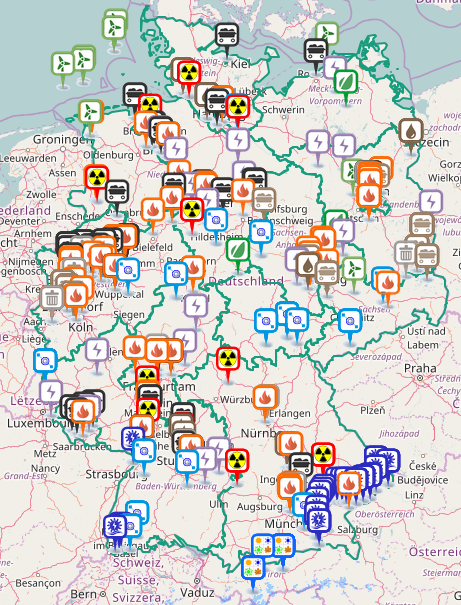
\includegraphics[width=.45\linewidth]{markers_new}}\hfill
\subfloat[Marker Cluster layer on Germany\label{markercluster}]
  {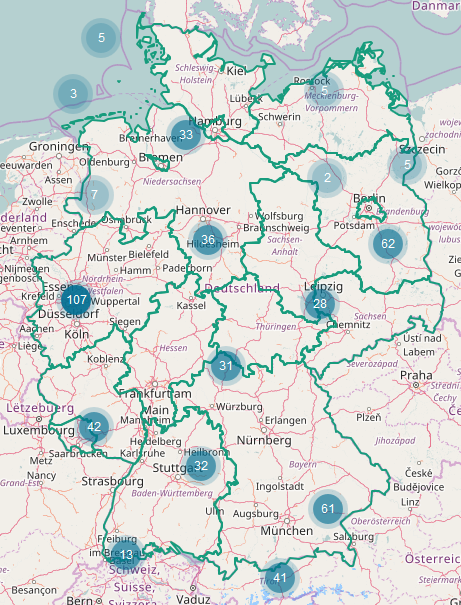
\includegraphics[width=.45\linewidth]{marker_cluster}}
\hfill
\caption{Impact of using marker cluster plugin}
\end{center}
\end{figure}

Figure \ref{marker} shows all the power plants with pinpoint marker inside Germany and Figure \ref{markercluster} shows the impact of using the marker cluster plugin. Clustered animated markers can be customized. Most importantly, it helps to visualize if there are more than one marker rendered in the same geographical location on the map. A cool built in feature spiderfies the child markers of that cluster. Figure \ref{fig:spiderfies} shows that there are in total 13 power plants located in the same area. Hence, to reduce complexity they are registered on a unique latitude and longitude.

\section*{Leaflet Label}

Leaflet label is a plugin for adding labels to markers \& different shapes such as paths, polygons, and circles on leaflet powered maps. \textbf{Leaflet.Label}\footnote{Github Leaflet.markercluster Website, \url{https://github.com/Leaflet/Leaflet.label/tree/0.2.1
} (last accessed on {\today})} development versions are available on GitHub . There is a default style for the label as you can see in the Figure \ref{fig:spiderfies} that power plants are located in Nordrhein-Westfalen. When the user hovers the cursor on the displayed objects of the map, this label appears with the data underlying for that particular object.

\begin{figure}[H]
  \begin{center}
\subfloat[Spiderfy view of multiple power plants located in the same location.
\label{fig:spiderfies}]
  {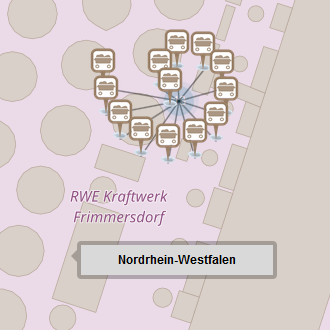
\includegraphics[width=.45\linewidth]{spider_new}}\hfill
\subfloat[Label of a Gas Power Plant\label{popupgas}]
  {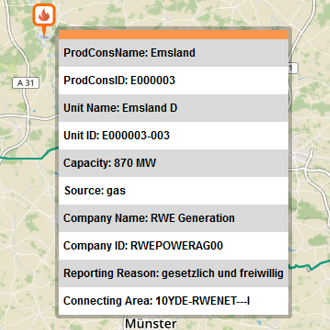
\includegraphics[width=.45\linewidth]{popupgas}}
\hfill
\caption{Impact of using marker cluster and Leaflet label plugin}
\end{center}
\end{figure}

\section*{jQuery}

jQuery is the most popular JavaScript library. Its features are rich. Its syntax is designed to make it easy for HTML document manipulation, handling events, animations, and developing Ajax applications. This free and open-source software enables developers for creating plugins on top of any JavaScript library. In our framework, jQuery is used for DOM element selection, manipulation and for handling events. For example, jQuery is used for the navigation menu in our framework. Our navigation menu is equipped with checkboxes and a drop-down menu. Effect of toggling checkboxes, the effect of selecting drop-down menu options, and handling these events on different zoom level are all handled by jQuery. The cross browser compatibility usage that makes jQuery even more a very helpful library. 
%Other applications of jQuery will be discussed in details in Chapter \ref{chap:softwareSystem}. 

\section*{Bootstrap}

Bootstrap is well known and free open-source framework. It is popular as front-end framework for designing websites. It is based on HTML \& CSS design with JavaScript extensions and dependent of jQuery. It provides a responsive structure to the website and compatible with almost all the latest versions of browsers. In our framework, we have used bootstrap to make our website responsive. In particular, it is incorporated for designing the navigation menu of our map.
Bootstrap buttons, check boxes and drop-down navigation menus styling provides a great performance on the websites. These components are interactive and made with JavaScript plugins which are bundled in the Bootstrap package. One of the main reasons to use this plugin is, it offers a good documentation for almost every element a typical web application requires. So it is easy to customize and understandable by any web developer. For creating a nice user-friendly interface for web applications with less effort, Bootstrap is a great solution.

\section{Working Environments}

Before developing the online visualization tool of German power plants the Fraunhofer Institute for Solar Energy Systems (ISE) was providing interactive charts on electricity production, electricity stock market prices and import/export of electricity at the website Energy Charts\footnote{Energy Chart official webpage, \url{http://www.energy-charts.de/} (last accessed on {\today})}. This whole framework is developed based on the libraries D3.js\footnote{d3.js official website, \url{https://d3js.org/} (last accessed on {\today})}  and NVD3.js footnote{NVD3.js official website, \url{http://nvd3.org/} (last accessed on {\today})} to interactively visualize the data in different chart types. Therefore, stacked area charts, multi bar charts, pie charts, chord diagrams as well as multi charts and discrete bar charts are used to present the data in a well understandable and user friendly way. The data that are presented in the charts are organized and stored in a structured way on the FTP server. The same web server is used for storing the data of power plants and power transmission lines as well as for storing the dependent libraries. The purpose of making these libraries available in the webserver is for fast loading times and maintain the compatibility of the tool.

%[language=json,firstnumber=1]
\begin{Listing}
\begin{lstlisting}
var Power_Plants = [
  { 
    "ProdConsName" : "Frimmersdorf",
    "ProdConsID" : "E000005",
    "UnitName" : "Frimmersdorf P",
    "UnitID" : "E000005-012",
    "Source" : "lignite",
    "color" : "rgb(150,125,100)" ,
    "Capacity" : 289,
    "CompanyName" : "RWE Generation",
    "CompanyID" : "RWEPOWERAG00",
    "ReportingAvailableCapacity" : "True",
    "WGS84Latitude" : 51.05629,
    "WGS84Longitude" : 6.57703,
    "Country" : "DE",
    "ReportingReason" : "gesetzlich und freiwillig",
    "ConnectingArea" : "10YDE-RWENET---I",
    "TSO" : "Amprion GmbH",
    "Commercialisation" : 1,
    "StartDate" : "2009-10-26T00:00:00+01:00",
    "EndDate" : "2017-09-30T00:00:00+02:00"
  },
  {....},
  {....}
]
\end{lstlisting}
\caption{An example of JSON-object for Brown Coal(lignite) power plant}
\label{lst:pp-json}
\end{Listing}

\section{File Format}
\label{sec:fileFormat}

All the data sources that have been used for power plant visualization and their production in the Energy Charts are in the JSON\footnote{JSON official website, \url{https://json.org/} (last accessed on {\today})}(JavaScript Object Notation) format. This is data format is language-independent and use the extension .json. The MasterData power file is received in CSV (Comma-separated values) format which is downloaded from the EEX\footnote{European Energy Exchange, \url{https://www.eex.com} (last accessed on {\today})} server. Fraunhofer ISE is authorized to download the files from the FTP server in CSV format and later it is converted into JSON data. List \ref{lst:pp-json} shows an example how power plant files are structured in JSON. 

%[language=json,firstnumber=1]
\begin{Listing}
\begin{lstlisting}
var _110KV_layer = [
    {
      "type": "Feature",
      "id": "way/18957128",
      "properties": {
        "@id": "way/18957128",
        "cables": "3",
        "frequency": "50",
        "power": "line",
        "voltage": "110000"
      },
      "geometry": {
        "type": "LineString",
        "coordinates": [
          [
            6.4336833,
            51.1353571
          ],
          [
            6.4337791,
            51.1353946
          ],
          [
            6.4345818,
            51.1357085
          ]
        ]
      }
    }
   ]
\end{lstlisting}
\caption{An example GeoJSON-object for 110kV power line inside Germany}
\label{lst:pl-json}
\end{Listing}

Another format that has been used for rendering power lines is GeoJSON\footnote{GeoJSON official website, \url{https://geojson.org/} (last accessed on {\today})}. It is a popular data format among GIS (Geographic Information System) technology and services. Leaflet is very good at handling both JSON and GeoJSON file format. Power lines are created from GeoJSON objects. According to \cite{geojson16}, GeoJSON object is a format for encoding a variety of geographic data structures in the form of geometry and collection of features. GeoJSON supports points, LineString, Polygon, Multipoint, MultiLineString, Multipolygon. Features in GeoJSON contain a geometry object and additional properties and a feature collection represents a list of features. The feature showed in the list \ref{lst:pl-json} belongs to the 110kV layer. Its geometry type is LineString and coordinates are given inside the geometry object. At the time of rendering, Leaflet generates a vector data layer from GeoJSON feature and adds it to the map.

\subsection{Advantage}

JSON is language independent, minimal, textual and subset of JavaScript  \cite{jsonfatfree2006}. This is one of the main reasons for using JSON. It is compatible with various JavaScript libraries, which really supports parsing JSON files. It is also compatible with browsers and web applications. JSON has a natural way of evolving the data and information. It is very simple to work with it in conjunction with the browser scripting. JSON can be imported into any website, it is smaller and can represent all Unicode characters. It's also trivial to use it in AJAX applications.
 
On the other hand, GeoJSON is also a data interchange format. It has a standardized way of passing information to the browser. Leaflet can adopt it well and its performance is very good compared to other available formats. It doesn't matter from where it was generated. As long as it is GeoJSON, users can render this on the map. It is also easily explorable because it can be handled in the same way as a regular JavaScript object. This furthermore offers a better handling of large files and even the easy use of filtering, styling and rendering on Leaflet by using this type.

\subsection{Disadvantage}

JSON is hard to read by a human and it is confusing. Its enormous number of braces, brackets, and commas made it almost unreadable. Therefore, sometimes it is difficult to generate a query for getting the target object from a complex JSON file. It is also not suitable for Big data.  An article \cite{jsontoobig} has described how big is too big for JSON.  Test results show that JSON file larger than 15MB is barely usable in modern browsers. Apparently, in our case, there was no underlying database implemented at the time of working. Hence, data are stored on the web server in the format of JSON or GeoJSON. Particularly, GeoJSON data of power lines are larger in size. Therefore, this large data files cause longer execution time for rendering. As a result, the browser crashes sometimes and performance of the map is affected after rendering a lot of polylines on the map. On the other hand, users would never be interested in downloading a large file which consumes so much data, especially on the mobile devices with limited bandwidth.

\begin{figure} [H]
  \begin{center}
    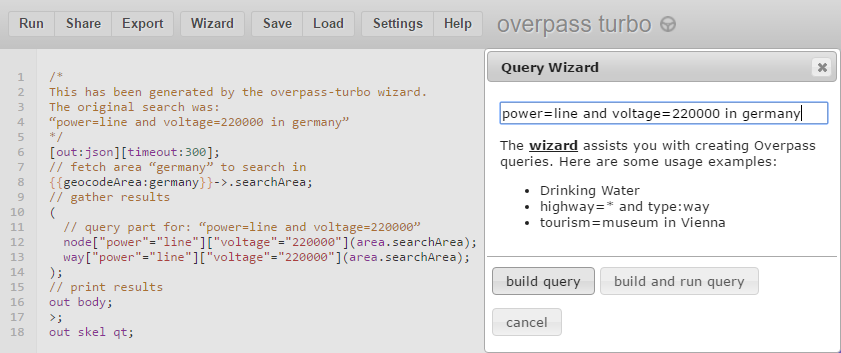
\includegraphics[width=1\textwidth]{wizardfull}
    \caption{Overpass turbo query wizard for generating query}
    \label{fig:wizard}
  \end{center}
\end{figure}

\section{Power line(GeoJSON) File Source}
\label{sec:plsource}

In this section, the source of GeoJSON data for power lines and how it is generated using Overpass turbo are discussed.
Power transmission line data are extracted from the overpass-turbo\footnote{Overpass turbo API, \url{https://overpass-turbo.eu/} (last accessed on {\today})} API. Overpass API acts like a database of OSM. It also offers search possibilities for viewing power lines on the OpenStreetMap. 

\begin{figure}
  \begin{center}
    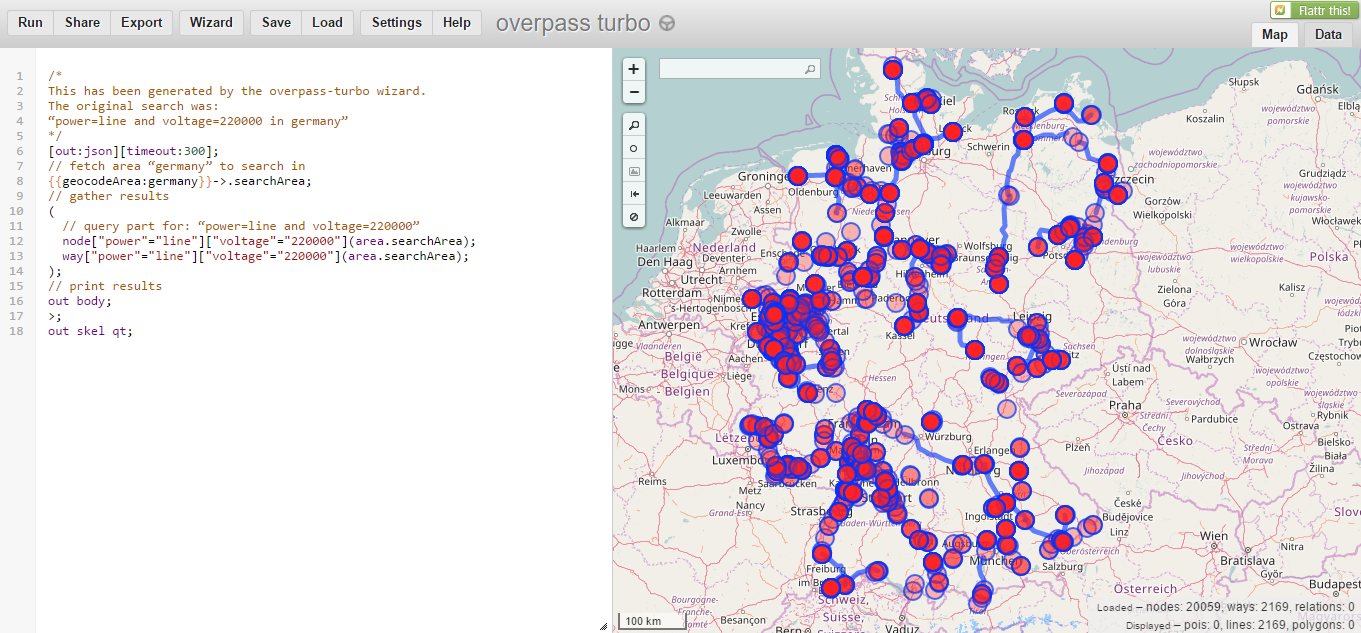
\includegraphics[width=1\textwidth]{optg}
    \caption[Overpass turbo API]{Overpass turbo API query (left) with rendered vector layer of 220kV power line (right) on the OpenStreetMap}
    \label{fig:optg}
  \end{center}
\end{figure} 

A unique tag value is used for querying power lines. The tag consists of two parts, one is a key and another is value. They are used together separated by an equal sign. Overpass API uses the tag and serves the part of the OSM map and render it on the map. Therefore, overpass turbo is used to run the overpass API query. There is a query wizard which assists in generating proper overpass query. An example is shown in the Figure \ref{fig:wizard}. To see power lines of 220kV, one has to fire up the wizard and enter \texttt{power=line}, \texttt{voltage=220000}. Here "power" is a key and "line" is a value for this tag. In addition, the fetch area of the map can be selected by mentioning it in the wizard or simply typing the name of the country next to \texttt{geocodeArea:} inside the curly brackets (see Figure \ref{fig:optg}, line 8).

After the execution of the query, filtered results are rendered on the OpenStreetMap. There is an option for exporting rendered data to various formats. We exported the data as GeoJSON and used it in our framework. This operation is done twice for exporting the GeoJSON of other two (110kV and 380kV) available power lines. The structure of this GeoJSON is already discussed in Section \ref{sec:fileFormat} on List \ref{lst:pl-json}.

 